\chapter{Event Selection}
\label{chapter:selection}

The \wztolnll{} decay is characterized by:
\begin{itemize}
\item a pair of same-flavor, opposite-charge, high-\pt, isolated leptons with an invariant mass consistent with a $Z$ boson,
\item a third high-\pt, isolated lepton, and
\item a significant deficit of transverse energy (\MET) associated with the escaping neutrino.
\end{itemize}
The selection criteria used for this analysis aim to identify $WZ$ events with as high an efficiency as possible while rejecting a significant fraction of background events with similar signatures.  The above characteristics can be supplemented by requirements related to the overall energy scale of the interaction for cases where the the $WZ$ pair originates from a massive resonance.  These criteria will be applied both to a measurement of the cross-section for SM $WZ$ production and to a search for a resonance in the $WZ$ spectrum, so there are certain places where the criteria diverge to provide optimal performance in different contexts, but the majority of the selection is uniform between the two measurements.

\section{Online Event Selection}
Over the course of 2011, CMS recorded \recordedlumi{} of $pp$ collision data, broken up into two major periods separated by a short technical stop.  
Each of the subsystems of the CMS detector experiences some amount of downtime due to equipment failures, meaning that some fraction of the recorded luminosity cannot be used for general analyses which rely on the integration of the full detector.  Consequently, the collaboration certifies a list of runs suitable for physics publication, which in the case of the 2011 data is equivalent to \jsonlumi.

Because the LHC delivers many more collisions than the CMS detector can record, the trigger system steps in to make quick decisions on which are worth keeping and which will not be as interesting for analysis.  The various triggers target different physics objects; among the many triggers available, one requires a single high-\pt electron, another requires a pair of electrons of intermediate \pt, and likewise for muons.  Since the events firing each type of trigger are generally independent, the data is naturally sorted into primary datasets (PDs) based on trigger type.

These primary datasets (and indeed the entire set of recorded data) are necessarily biased in favor of events with certain content.  This bias has potential repercussions for physics results and must be considered when constructing an analysis.  To ensure a sufficient understanding of the online selection, some portion of each analysis effort goes into carefully measuring the efficiency for events of interest to fire the relevant triggers and incorporating that information into the final result.  Often, this means not only choosing some small number of datasets for the selection of signal events, but also an additional set with different biases to allow the efficiency measurements.

For this analysis, we consider the \texttt{DoubleElectron} and \texttt{DoubleMu} datasets where events must fire a trigger looking for a pair of electrons or a pair of muons, respectively.  To control the recorded event rate, each of these triggers imposes energy thresholds on the candidate objects, with these thresholds increasing as the luminosity has increased.  These HLT paths are each seeded by a Level-1 trigger path requiring one or two low-level detector objects with thresholds lower than those imposed at higher levels.  The thresholds corresponding to various run ranges are given in Table~\ref{tab:trigger-thresholds}.

\begin{table}
  \centering
  \begin{tabular}{c r r r r r r r r}
    \toprule
    % & \multicolumn{8}{c}{Thresholds/\GeV} \\ \cmidrule{2-9}
    & \multicolumn{4}{c}{$\et(e^\pm)$/(\GeV)} & \multicolumn{4}{c}{$\pt(\mu^\pm)$/(\GeVc)} \\ \cmidrule(r){2-5} \cmidrule(l){6-9}
    Run Range & \multicolumn{2}{c}{L1} & \multicolumn{2}{c}{HLT} & \multicolumn{2}{c}{L1} & \multicolumn{2}{c}{HLT} \\ 
    %\midrule
    \cmidrule(r){1-1} \cmidrule(rl){2-3} \cmidrule(rl){4-5} \cmidrule(rl){6-7} \cmidrule(l){8-9}
    160329--164236 & 12 & --- & 17 & 8 & 3 & 3 &  7 & 7 \\
    165088--170759 & 12 & --- & 17 & 8 & 3 & 3 & 13 & 8 \\
    170826--178380 & 12 &   5 & 17 & 8 & 3 & 3 & 13 & 8 \\
    178420--180296 & 12 &   5 & 17 & 8 & 3 & 3 & 17 & 8 \\
    \bottomrule
  \end{tabular}
  \caption[Trigger thresholds]{Thresholds for the double electron and double muon triggers used in this analysis.  The Level-1 seed for the electron triggers initially requires only one object with $\et > \sienergy{12}$, but later requires an additional deposit with $\et > \sienergy{5}$.}
  \label{tab:trigger-thresholds}
\end{table}

\section{Electron Selection}
\label{sec:electron-selection}
Although previous experiments have developed multivariate discriminators to provide optimal efficiency in identifying high-quality electrons, this analysis chooses a simpler cut-based approach.  This choice reflects both the necessity to build understanding of lepton identification during the first year of full LHC operation and the excellence of the CMS detector that in most analyses makes complicated multivariate lepton identification unnecessary.  We define a separate set of requirements for each of the three lepton roles, with the requirements on an electron associated with the $W$ significantly tighter than those for the $Z$ leptons.  Whereas the invariant mass constraint on the $Z$ leads to a relatively pure sample of $Z$ bosons, there is a high probability to choose a jet when searching for a $W \to e + \nu$ decay.  The selection criteria are specifically chosen to reduce the frequency of jets entering into the pool of electron candidates.

Electrons assigned to a $Z$ decay are required to match objects passing the double electron trigger.  The matching compares the $(\eta, \phi)$ coordinates of the reconstructed electrons and the electron objects identified in the HLT, requiring $\Delta R < 0.1$ (see Eq.~\ref{eq:deltar}).  In order to ensure a high trigger efficiency, we must impose \et requirements on the reconstructed electrons such that they lie on the plateau of the trigger efficiency curve with respect to electron \et.  To match the trigger thresholds of \sienergy{17} and \sienergy{8}, the leading electron must have $\et > \sienergy{20}$ while the other may have \et as low as \sienergy{10}.

All electrons must be within the detector acceptance ($|\eta| < 2.5$) and meet several criteria testing the compatibility of the electromagnetic shower shape with the isolated electron hypothesis.  The shower is evaluated for the width of the electromagnetic cluster in terms of pseudorapidity ($\sigma_{i\eta i\eta}$ where $i$ indicates that the measurement is taken as a number of crystals rather than a distance, see Sec.~\ref{sec:ecal}), the difference in the measured position of the \ecal supercluster vs.\ the associated track ($\Delta\phi$ and $\Delta\eta$), and the ratio of energy deposited in the \ecal vs.\ the \hcal ($E_\text{HCAL} / E_\text{ECAL}$).  Because calorimeter response differs significantly between the barrel and the endcap, the values for these criteria are determined separately for these two regions.  Table~\ref{tab:electron-requirements} gives the specific values for all electron requirements applied in this analysis with the corresponding distributions shown in Fig.~\ref{fig:electron-cuts-hb} for candidates in the barrel region and Fig.~\ref{fig:electron-cuts-he} for candidates in the endcap region.

\begin{table*}
  \centering
  \begin{tabular}{rrrrrrr}
    \toprule
    & \multicolumn{2}{c}{Electrons from $Z$} & \multicolumn{2}{c}{Electron from $W$} \\ \cmidrule(r){2-3} \cmidrule(l){4-5}
    Requirement & EB & EE & EB & EE \\
    \midrule
    Minimum trigger match \et (\GeV) & 17 (8) & 17 (8) & --- & --- \\
    Minimum electron \pt (\GeVc) & 20 (10) & 20 (10) & 20 & 20 \\
    Maximum $\sigma_{i\eta i\eta}$ & 0.012 & 0.031 & 0.010 & 0.031 \\
    Maximum $|\Delta\eta_\text{in}|$ & 0.007 & 0.011 & 0.005 & 0.006 \\
    Maximum $|\Delta\phi_\text{in}|$ & 0.800 & 0.700 & 0.027 & 0.021 \\
    Maximum missing track hits & 0 & 0 & 0 & 0 \\
    Minimum $d$ between tracks (\si{cm})& --- & --- & 0.02 & 0.02 \\
    Minimum $\Delta\cot(\theta)$ between tracks & --- & --- & 0.02 & 0.02 \\
    Maximum $R_\text{iso}$ & 0.15 & 0.10 & 0.07 & 0.06 \\
    Minimum $\Delta R$ from any muon & 0.01 & 0.01 & 0.01 & 0.01 \\
    \bottomrule
  \end{tabular}
  \caption[Requirements imposed on electrons]{Requirements imposed on electrons.  The first two rows give criteria applied to the more energetic $Z$ electron first, with the value for the less energetic electron in parentheses.}
  \label{tab:electron-requirements}
\end{table*}

\begin{figure*}[p]
  \centering
  \newcommand{\mywidth}{0.47\textwidth}
  \newcommand{\mygraph}[1]{\includegraphics[width=0.49\textwidth]{matplotlib/#1.\figext}}
  \mygraph{lepcuts100/hb_pt}\hfill\mygraph{lepcuts10/hb_iso}\\
  \mygraph{lepcuts100/hb_detain}\hfill\mygraph{lepcuts100/hb_dphiin}\\
  \mygraph{lepcuts100/hb_nmiss}\hfill\mygraph{lepcuts100/hb_sieie}\\
  \mygraph{lepcuts100/hb_dist}\hfill\mygraph{lepcuts100/hb_dcot}\\
  \caption[Distributions of criteria used to select barrel electrons]{Distributions of criteria used to select barrel electrons, considering all remaining candidates with $\et > \sienergy{20}$ after a \ztoll{} decay is identified.  Collision data (composed mostly of jets) is compared to simulated $WZ$ events (composed mostly of true electrons) to show the discriminating power of each requirement.  Shaded areas indicate excluded regions; when two different depths of shading are used, the lighter one indicates a region of conditional exclusion as described in Table~\ref{tab:electron-requirements}.}
  \label{fig:electron-cuts-hb}
\end{figure*}

\begin{figure*}[p]
  \centering
  \newcommand{\mywidth}{0.47\textwidth}
  \newcommand{\mygraph}[1]{\includegraphics[width=0.49\textwidth]{matplotlib/#1.\figext}}
  \mygraph{lepcuts100/he_pt}\hfill\mygraph{lepcuts10/he_iso}\\
  \mygraph{lepcuts100/he_detain}\hfill\mygraph{lepcuts100/he_dphiin}\\
  \mygraph{lepcuts100/he_nmiss}\hfill\mygraph{lepcuts100/he_sieie}\\
  \mygraph{lepcuts100/he_dist}\hfill\mygraph{lepcuts100/he_dcot}\\
  \caption[Distributions of criteria used to select endcap electrons]{Distributions of criteria used to select endcap electrons, considering all remaining candidates with $\et > \sienergy{20}$ after a \ztoll{} decay is identified.  Collision data (composed mostly of jets) is compared to simulated $WZ$ events (composed mostly of true electrons) to show the discriminating power of each requirement.  Shaded areas indicate excluded regions; when two different depths of shading are used, the lighter one indicates a region of conditional exclusion as described in Table~\ref{tab:electron-requirements}.}
  \label{fig:electron-cuts-he}
\end{figure*}

Photons originating from a hard interaction have a high probability to convert to an $e^+e^-$ pair within the tracker.  Those tracks, however, are likely to be missing hits in the innermost regions, so we can discriminate against them by requiring that electron tracks have no missing hits.  Electrons assigned to a $W$ decay are also checked for extra tracks in their immediate vicinity and rejected if any fall within a distance $d$ of \SI{0.2}{mm} or are not sufficiently separated to satisfy $\Delta\cot(\theta) < 0.02$.

For isolation, we take the approach of drawing a cone (defined as $\Delta R < 0.3$) around each electron and looking for objects inside that cone.  The objects considered include tracks in the inner tracker where the cone is defined around the electron track's position from the origin as well as calorimeter deposits where the cone is defined around the electron's location at the inside surface of the \ecal.  Isolation is quantified as a sum of the transverse energies of all tracks and calorimeter deposits within those cones which are not associated with the electron:
\begin{equation}
  \label{eq:isolation}
  \et^\text{iso} = c \cdot \!\!\!\sum_i^\text{tracker}\!\!\! \pt(i) + \!\!\!\sum_i^\text{ECAL}\!\!\! \et(i) + \!\!\!\sum_i^\text{HCAL}\!\!\! \et(i).
\end{equation}
In order to allow a high acceptance for energetic electrons, we set a requirement not on the isolation sum itself, but rather on the ratio of the isolation sum to the electron's transverse momentum:
\begin{equation}
  \label{eq:riso}
  R_\text{iso} = \frac{\et^\text{iso}}{c \cdot \pt}.
\end{equation}

\begin{figure*}[!htbp]
  \centering
  \subbottom[Before correction.]{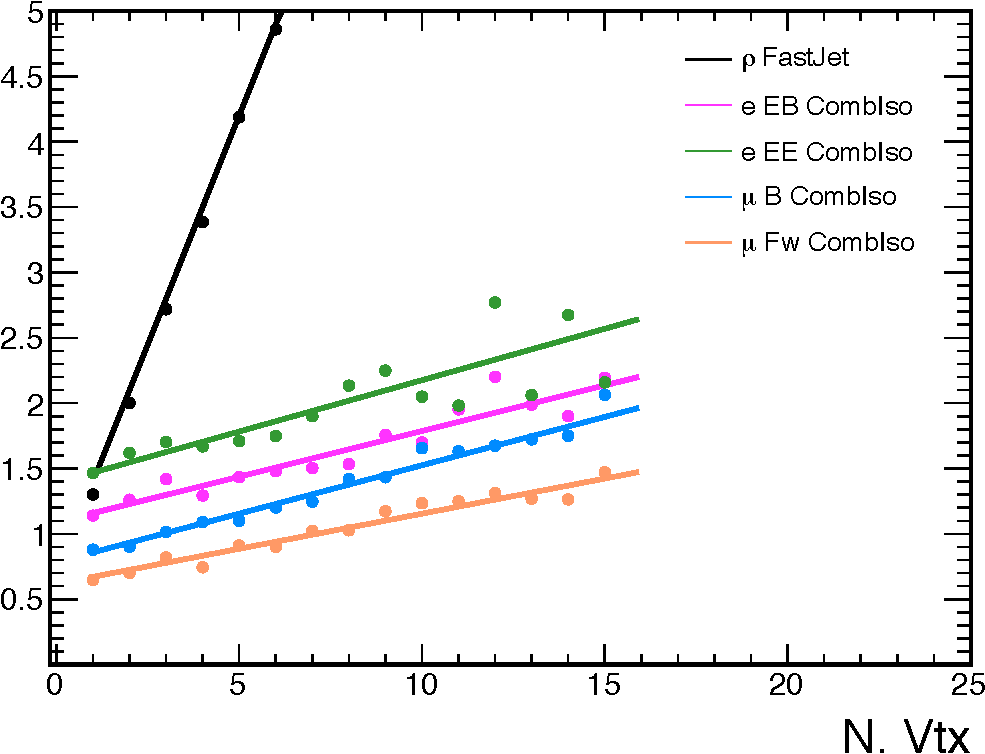
\includegraphics[width=0.47\textwidth]{figures/fastjet-before-crop}\label{fig:fastjet-before}}
  \hfill
  \subbottom[With correction applied.]{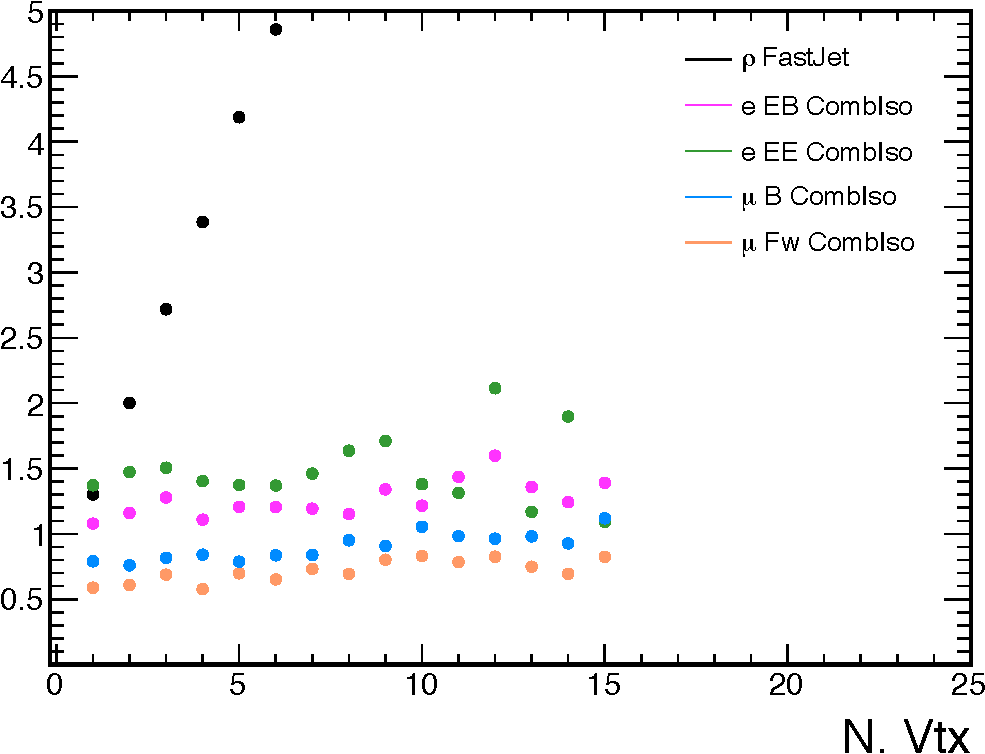
\includegraphics[width=0.47\textwidth]{figures/fastjet-after-crop}\label{fig:fastjet-after}}
  \caption[Mean values of the combined isolation sum as a function of the number of reconstructed primary vertices, before and after the pileup correction]{Mean values of the combined isolation sum as a function of the number of reconstructed primary vertices, before and after the pileup correction.  The black line is a fit to the estimated energy density due to pileup.}
  \label{fig:fastjet-correction}
\end{figure*}

The isolation sum is sensitive to pileup effects since additional interactions lead to more jet activity in the event.  To ensure a stable efficiency for the isolation requirement with respect to pileup, the isolation sum is corrected based on the \textsc{fastjet} determination of the energy density $\rho$ due to pileup and the underlying event.  The isolation sum is reduced according to the measured diffuse noise $\rho$ in the event, with effects shown in Fig.~\ref{fig:fastjet-correction}.

One final, though small, concern for electron identification comes from cases where photons are generated from internal \brem{} in $W$ and $Z$ decays, closely aligned with one of the resulting leptons.  If produced near an electron, such a photon will likely be correctly included as part of the electron's supercluster in the \ecal; if produced near a muon, however, it likely to be misidentified as a distinct electron.  To remove these ambiguities, electrons found in the immediate vicinity of a muon ($\Delta R < 0.01$) are rejected.

Detailed efficiency measurements discussed later in this chapter (see Sec.~\ref{sec:lepton-selection-efficiency}) give an overall efficiency of 73\% for an electron produced by a $W$ decay to pass our selection.  
We can investigate the misidentification rate in simulation by looking at a sample of \Zjets{} events with a \ztomumu{} decay such that all reconstructed electrons should be due to misidentified jets.  Considering all reconstructed jets and electrons with $\et > \sienergy{20}$, we find that 0.9\% of jets result in a basic electron object, with only 11\% of those passing the full $W$ decay identification and isolation criteria. 


\section{Muon Selection}
\label{sec:muon-selection}
The muon selection follows a requirement-based approach similar to that used for electrons.  Muons are restricted to be within the pseudorapidity acceptance ($|\eta| < 2.4$) of the muon and tracking systems and to fulfill various track quality requirements.  The global track fit must contain at least eleven inner tracker hits including one or more hits in the pixel detector and at least one hit in the muon system.  Moreover, the muon must be matched to track segments in two different muon stations.  In order to reject muons from hadrons decaying in flight or from kaons punching through the calorimeter, the overall quality of the global muon fit must be high as measured by a requirement on the normalized $\chi^2$ (meaning that we divide the $\chi^2$ value by the number of degrees of freedom in the fit).  To reject cosmic ray muons which do not originate from a collision, we also require that the impact parameter of the global fit with respect to the measured beam spot be less than \SI{2}{mm}.  These track quality requirements are shown in Table~\ref{tab:muon-requirements} along with the isolation values.

\begin{table*}
  \centering
  \begin{tabular}{r rrr}
    \toprule
    \multicolumn{3}{r}{Minimum number of pixel hits} & 1 \\
    \multicolumn{3}{r}{Minimum number of tracker hits} & 11 \\
    \multicolumn{3}{r}{Minimum number of muon system hits} & 1 \\
    \multicolumn{3}{r}{Minimum number of matched muon segments} & 2 \\
    \multicolumn{3}{r}{Maximum normalized $\chi^2$} & 10.0 \\
    \multicolumn{3}{r}{Maximum impact parameter (cm)} & 0.2 \\
    \midrule
    & $\mu^Z_1$ & $\mu^Z_2$ & $\mu^W$ \\ \cmidrule{2-4}
    Minimum trigger match \pt (\GeVc) & 17 & 8 & --- \\
    Minimum global track \pt (\GeVc) & 20 & 10 & 20 \\
    Maximum $R_\text{iso}$ & 0.15 & 0.15 & 0.10 \\
    \bottomrule
  \end{tabular}
  \caption[Requirements imposed on muons]{Requirements imposed on muons.  The first six rows apply to all muons considered for the analysis while the values in the final three rows take into account the specific role for which a muon has been selected.  The requirements under the headings $\mu^Z_1$ and $\mu^Z_2$ are applied to the higher-\pt and lower-\pt legs of a \ztomumu{} decay while the requirements under the heading $\mu^W$ are applied to muons assigned to a \wtomunu{} decay.}
  \label{tab:muon-requirements}
\end{table*}

\begin{figure*}[p]
  \centering
  \newcommand{\mygraph}[1]{\includegraphics[width=0.49\textwidth]{matplotlib/#1.\figext}}
  \mygraph{lepcuts100/hm_pt}\hfill\mygraph{lepcuts10/hm_iso}\\
  \mygraph{lepcuts10/hm_npix}\hfill\mygraph{lepcuts10/hm_ntrk}\\
  \mygraph{lepcuts10/hm_nmuo}\hfill\mygraph{lepcuts10/hm_nseg}\\
  \mygraph{lepcuts10/hm_chi2}\hfill\mygraph{lepcuts10/hm_d0}\\
  \caption[Distributions of criteria used to select muons]{Distributions of criteria used to select muons, considering all remaining candidates with $\pt > \simomentum{20}$ after a \ztoll{} decay is identified.  Collision data (composed mostly of jets) is compared to simulated $WZ$ events (composed mostly of true muons) to show the discriminating power of each requirement.  Shaded areas indicate excluded regions; the lighter shaded region in the $R_\text{iso}$ distribution is excluded only when considering a \wtomunu{} decay.}
  \label{muon-cuts}
\end{figure*}

Isolation for muons is exactly analogous to the algorithm for electrons (Eqs.~\ref{eq:isolation} and~\ref{eq:riso}) again with the transverse momenta and energies summed in separate $\Delta R$ cones of radius 0.3 for the tracker, \ecal, and \hcal.  Again, contributions from the muon in question are removed.  The same pileup correction is applied, depending on the number of reconstructed vertices in the event and the region of the detector in which the muon is found.

The selection used for muons is identical for those assigned to a $W$ decay vs.\ those assigned to a $Z$ decay except for a tighter isolation requirement on the $W$ and a trigger matching requirement on both muons assigned to a $Z$ decay.  As with electrons, our primary concern for muon identification is to reduce the possibility for a jet to included as a lepton in the $W$ decay where we are not protected by an invariant mass constraint.  Trigger matching and \pt cuts are exactly analogous to the electron case.

Detailed efficiency measurements discussed later in this chapter (see Sec.~\ref{sec:lepton-selection-efficiency}) give an overall efficiency of 86\% for a muon produced by a $W$ decay to pass our selection.  
We can investigate the misidentification rate in simulation by looking at a sample of \Zjets{} events with a \ztoee{} decay such that all reconstructed muons should be due to misidentified jets.  Considering all reconstructed jets with $\et > \sienergy{20}$ and all reconstructed muons with $\pt > \simomentum{20}$, we find that 0.003\% of jets result in a muon object, with only 0.6\% of those passing the full $W$ decay identification and isolation criteria.

\section{Final Selection of \textit{WZ} Candidates}
$Z$ boson candidates are built from a pair of opposite-sign, same-flavor leptons with \pt and trigger matching requirements as discussed in Secs.~\ref{sec:electron-selection} and~\ref{sec:muon-selection} along with an invariant mass between \simass{60} and \simass{120}.  If the available leptons produce more than one such combination, we choose the one most consistent with the nominal $Z$ mass.  If, however, four or more leptons are present which can yield two distinct $Z$ candidates, the event is rejected to suppress $ZZ$ background.

We assign the highest-\pt candidate from the remaining leptons to the $W$ boson decay.  The transverse mass of the $W$ boson candidate $\mt(W)$ is given as:
\begin{equation}
  \label{eq:wtransmass}
  \mt(W) \equiv \sqrt{2 \cdot \MET \cdot \pt(\ell) \cdot \Delta \phi}
\end{equation}
with $\pt(\ell)$ the transverse momentum of the lepton assigned to the $W$ and $\Delta \phi$ the angle between that lepton and the \MET in the transverse plane.  Distributions showing $M(Z)$, \MET, and $\mt(W)$ after selection of the third lepton are shown in Figs.~\ref{fig:validw-zmass}, \ref{fig:validw-met}, and~\ref{fig:validw-transmass}.  

To reject a large fraction of events without a genuine $W$ decay, we require that the \MET calculated from particle flow be above \sienergy{30}, indicating the recoil of a high-energy neutrino.

\begin{figure}
  \centering
  \includegraphics[width=\plotwidth]{matplotlib/hZMass_ValidW}
  \caption{Reconstructed mass of the $Z$ boson candidate for events with an extra isolated lepton passing requirements for the $W$.}
  \label{fig:validw-zmass}
\end{figure}

\begin{figure}
  \centering
  \includegraphics[width=\plotwidth]{matplotlib/hMET_ValidW}
  \caption{Distribution of missing transverse energy for events with a valid $Z$ candidate and an extra isolated lepton passing requirements for the $W$.}
  \label{fig:validw-met}
\end{figure}

\begin{figure}
  \centering
  \includegraphics[width=\plotwidth]{matplotlib/hWTransMass_ValidW}
  \caption{Transverse mass of the $W$ boson candidate for events with a valid $Z$ candidate and an extra isolated lepton passing requirements for the $W$.}
  \label{fig:validw-transmass}
\end{figure}

Massive exotic particles decaying via $WZ$ should be most easily distinguished from the SM $WZ$ background by virtue of a narrow width in the spectrum of the system's reconstructed mass $M(WZ)$.  That mass, however, depends on the longitudinal momentum $p_z$ of the neutrino, which cannot be inferred from the information recorded by the detector.  We proceed by assuming the $W$ to have its nominal mass, leading to a quadratic equation with $p_z(\nu)$ the only unknown.  As long as the reconstructed $\mt(W)$ lies below the nominal $W$ mass, this equation yields two real solutions.  We choose the lower magnitude of the two $p_z(\nu)$ solutions as it is found to give the $M(WZ)$ value more consistent with the generator-level $WZ$ mass in 75\% of simulated events.  Due to the finite detector resolution, some fraction of events ($\approx$ 20\%) yield a reconstructed value of $\mt(W)$ which exceeds the nominal $W$ mass and generates complex results in the $p_z(\nu)$ equation
% (see Fig.~\ref{fig:complex-angle})
.  
In these cases, we replace the $M(W)$ assumption with the measured transverse mass, recovering a unique real solution.

In addition to the invariant mass distinction, we expect that $WZ$ events originating from the decay of a massive particle should in general be more energetic than the events expected from the Standard Model.  We quantify this by considering the scalar sum of the transverse momenta of the final state leptons:
\begin{equation}
  \label{eq:lepht}
  \lepht = \sum_i \pt(\ell_i),
\end{equation}
where $i$ iterates over the three charged leptons associated with the \ztoll and \wtolnu decays.

% \begin{figure}
%   \centering
%   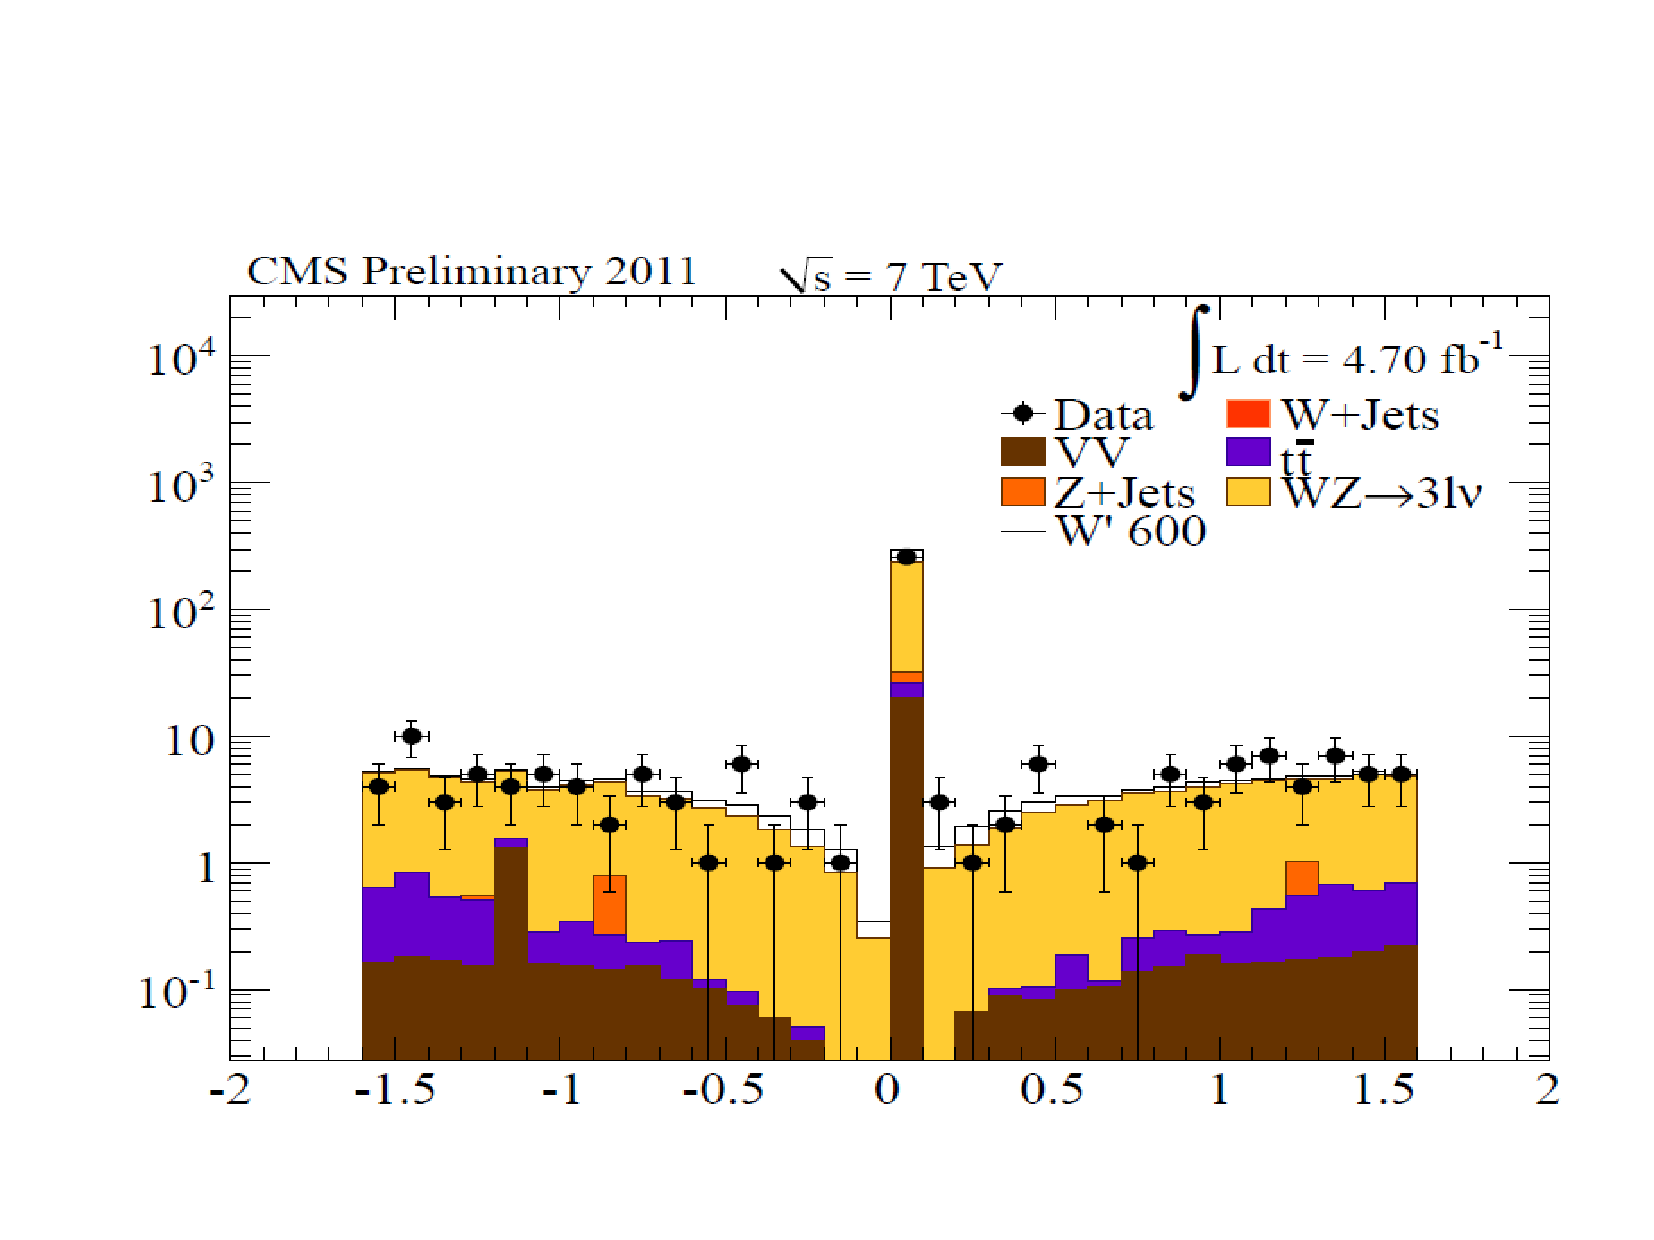
\includegraphics[width=\plotwidth]{figures/plot-complex-angle}
%   \caption{Distribution of the complex angle for the potential solutions to the quadratic equation for $p_z(\nu)$ under the nominal $M(W)$ assumption.  The large central peak corresponds to real solutions with fewer than 5\% of events having an imaginary component.}
%   \label{fig:complex-angle}
% \end{figure}

% We define the transverse mass of the $WZ$ system~\cite{Belyaev:2007ss}:
% \begin{equation}
%   \label{eq:wzmt}
%   M^2_\text{T}(WZ) = (\sqrt{M^2(\ell\ell\ell) + \pt^2(\ell\ell\ell)} + |\MET|)^2 -|\pt(\ell\ell\ell) + \MET|^2. 
% \end{equation}

We use requirements on the $M(WZ)$ and \lepht distributions to achieve further separation between resonant particles and SM $WZ$ production.  The mass windows and minimum \lepht values are determined separately for each simulated mass point, optimizing for the best expected limit.  The distributions of \lepht and invariant mass for selected $WZ$ candidates are shown in figures~\ref{fig:ht} and~\ref{fig:mwz}.

\begin{figure}
  \centering
  \includegraphics[width=\plotwidth]{matplotlib/hHt_ValidWZCand}
  \caption{Distribution of \lepht in simulated samples and collision data.}
  \label{fig:ht}
\end{figure}

\begin{figure}
  \centering
  \includegraphics[width=\plotwidth]{matplotlib/hWZMass_ValidWZCand}
  \caption{Distribution of $WZ$ invariant mass in simulated samples and collision data.}
  \label{fig:mwz}
\end{figure}

\section{Optimization of Analysis Cuts}
The selection criteria for the $W$ and $Z$ bosons, including identification and isolation of the constituent leptons, provide sufficient suppression of all background except for the genuine $WZ$ events predicted in the Standard Model.  The requirements on $M(WZ)$ and \lepht, then, are motivated by a desire to distinguish exotic particles from SM $WZ$.  Both of these requirements capitalize on the rapid suppression of the SM cross section with increasing mass beyond the threshold value of \simass{170}.  Although a mass window alone could provide significant power to discriminate against SM events, the mass resolution is poor due to its dependence on inferences about the escaping neutrino.  In comparison, the \lepht measurement plays to the strengths of the CMS detector in electron and muon reconstruction, thus providing a more reliable gauge of how energetic the system may be.  The complementary nature of these two requirements is illustrated in Fig.~\ref{fig:mass-vs-ht}.

\begin{figure}
  \centering
  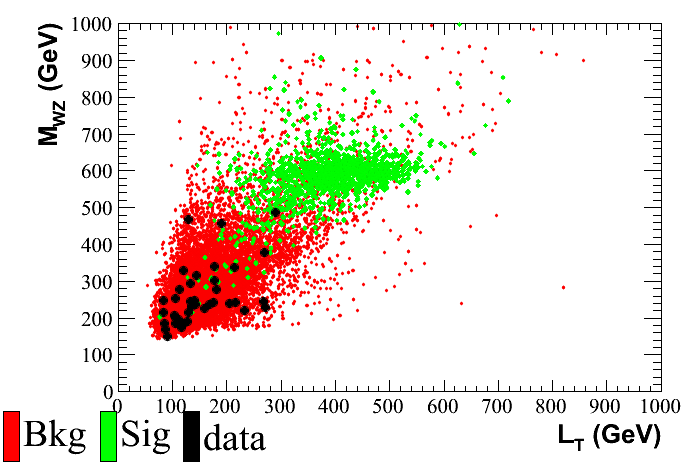
\includegraphics[width=\plotwidth]{figures/plot-mass-vs-lt.png}
  \caption[Distribution of \lepht vs. $M(WZ)$ for a \simass{600} \wprime signal sample and for $WZ$ background]{Distribution of \lepht vs. $M(WZ)$ for a \simass{600} \wprime signal sample and for $WZ$ background.  Because the samples have a significant width with respect to both parameters, substantial sensitivity gains can be achieved through a combined requirement.}
  \label{fig:mass-vs-ht}
\end{figure}

The \lepht requirements and mass windows are optimized simultaneously.  The minimum \lepht is initially set to \simomentum{50} (the minimum possible value based on the lepton \pt requirements) and increased in increments of \simomentum{10}, in line with the lepton \pt resolution.  The mass window is symmetric and centered on the nominal mass of the $WZ$ system, expanding outward in steps of \simass{10} on either side.

The requirements can be optimized with respect to various figures of merit, often some ratio between the number of signal and background events passing the selection.  We choose a full calculation of the expected limit (described in Sec.~\ref{sec:limit-technique}) for each potential mass window plus \lepht pairing as our figure of merit, choosing the combination which gives the best limit.  Due to diminishing background statistics at high $M(WZ)$, errors on the expected limit become large enough that no meaningful optimization of the \lepht requirement can be made, so we keep the requirement optimized for an \simass{800} signal when considering higher mass ranges.  The optimized requirements for each mass point are presented along with final event yields and cross section limits in Table~\ref{tab:event-yields}.  This simultaneous approach provides a marginal improvement over previous techniques which used functions of the signal and background yields to optimize the \lepht requirement and the mass window sequentially.

\section{Efficiency of Lepton Selection}
\label{sec:lepton-selection-efficiency}
We determine the efficiency of our electron and muon selection criteria by applying a ``tag and probe'' measurement to each stage of the selection.  This method exploits the $Z \to e^+ + e^-$ and $Z \to \mu^+ + \mu^-$ resonances to provide a sample of real leptons that is unbiased with respect to the quantities being measured.  The approach involves selecting events with a ``tag'' lepton passing some tight selection, then searching for a ``probe'' lepton which forms an invariant mass consistent with a $Z$ boson when paired with the tag.  Due to the mass constraint, this sample of probes can be assumed to consist almost entirely of real leptons.  If we consider our selection criteria as a series of sequential requirements, then the efficiency of a particular step is given by the fraction of probes passing all previous criteria which also pass the requirement in question.

\begin{figure*}
  \centering
  \subbottom[electrons]{\includegraphics[width=0.49\textwidth]{matplotlib/efficiencies/turnon-electron}}
  \hfill
  \subbottom[muons]{\includegraphics[width=0.49\textwidth]{matplotlib/efficiencies/turnon-muon}}
  \caption[Efficiencies for isolated electrons and muons to pass the trigger requirement as a function of \pt]{Efficiencies for well-identified, isolated (a) electrons and (b) muons (right) to pass the trigger requirement as a function of the lepton's transverse momentum.  In both cases, the trigger requires an object with $\pt > \simomentum{17}$, leading to a ``turn-on'' region with respect to the higher-resolution \pt measurement used in offline reconstruction.  The requirement that $\pt > \simomentum{20}$ on the leading reconstructed lepton assigned to the $Z$ decay is chosen to ensure all candidates are on or near the plateau of the above efficiency curves.}
  \label{fig:trigger-turnon}
\end{figure*}

These tag and probe measurements are applied to both collision data and Monte Carlo simulation in order to determine ratios which can be used to correct the event yields in simulation.  For the trigger efficiency measurements in data, special care is taken to select events from single-lepton datasets where the tag is matched to the trigger so as not to introduce a trigger bias.  For electron measurements, we use a special path designed specifically for tag and probe studies which requires a single electron object with $\et > \sienergy{17}$ along with a supercluster in the \ecal with $\et > \sienergy{8}$.  As the supercluster-finding efficiency is nearly 100\%, this requirement introduces little bias to the efficiency and identification measurements.

Results are extracted from the tag and probe samples through functional fits to the invariant mass of tag-probe pairs.  The $Z$ peak is fit with a Gaussian multiplied by an exponential to allow a low-end tail while the non-peaking background is assumed to be linear, with the resulting fit subtracted from the peak.  A systematic uncertainty is estimated for each measurement by replacing the function used to fit the $Z$ peak with other possible shapes such as a Gaussian multiplied by a quadratic.  The variation in the extracted efficiency with respect to different fitting functions is in most of these measurements less than 0.5\%.  These errors are factored into the final results as discussed in Sec.~\ref{sec:systematics}.

The observed efficiencies show various levels of dependence on the transverse momentum and pseudorapidity of the lepton.  In the trigger case, the efficiency has a sharp dependence on \pt in the immediate vicinity of the trigger threshold, but quickly reaches a plateau of near constant efficiency, as shown in Fig.~\ref{fig:trigger-turnon}.  The \pt requirements on reconstructed leptons for this analysis are chosen so as to avoid this ``turn-on'' region of the trigger efficiency curve.  For other measurements, the momentum and pseudorapidity dependence is small within the population of leptons considered in this analysis.  Because the sensitivity gains from a binned efficiency measurement would be negligible, we make a single measurement for each efficiency which represents the entire range of leptons considered.

\begin{table*}[p]
  \newcommand{\sep}{$\,\pm\,$}
  \centering
  \begin{tabular}{l l@{\sep}r l@{\sep}r l@{\sep}r}
    \toprule
    Efficiency & \multicolumn{2}{c}{Data/\%} & \multicolumn{2}{c}{MC/\%} & \multicolumn{2}{c}{Ratio ($\frac{\text{Data}}{\text{MC}}$)} \\
    \midrule
    Identification \hfill($W$) & 84.8&0.1 & 84.9&0.1 & 0.999&0.001 \\
    Isolation \hfill($W$)      & 85.6&0.1 & 81.7&0.1 & 1.047&0.002 \\
    Identification \hfill($Z$) & 97.4&0.1 & 97.6&0.1 & 0.998&0.001 \\
    Isolation \hfill($Z$)      & 97.9&0.1 & 97.3&0.1 & 1.006&0.001 \\
    Trigger \hfill($\et > \sienergy{17}$) & 95.8&0.1 & 98.2&0.1 & 0.976&0.001 \\
    Trigger \hfill($\et > \sienergy{08}$) & 95.8&0.1 & 98.2&0.1 & 0.976&0.001 \\
    \bottomrule
  \end{tabular}
  \caption[Electron efficiency values obtained from the tag and probe
fits]{Electron efficiency values obtained from the tag and probe
fits.  For each efficiency, we give the value obtained from data, the
value obtained from MC simulation, and the ratio of data to MC.  The
errors quoted are purely statistical.}
\label{tab:electron-efficiencies}
\end{table*}

\begin{figure*}[p]
  \centering
  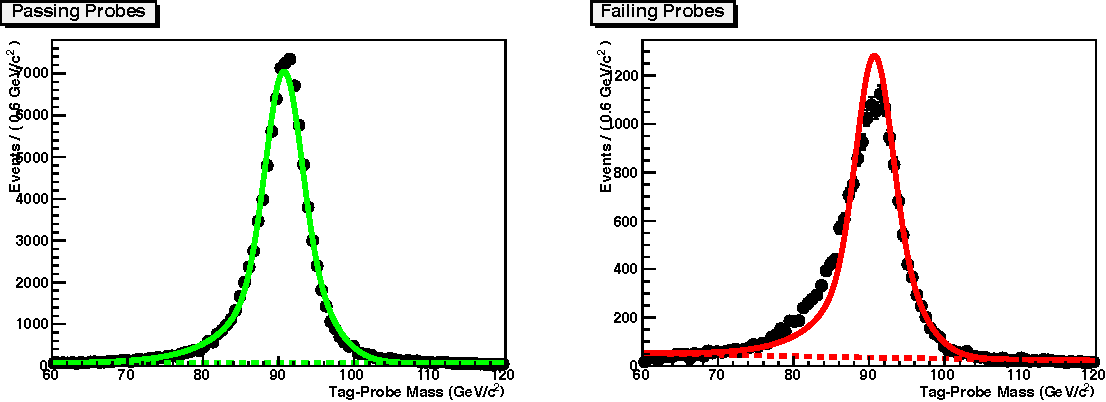
\includegraphics[width=\textwidth,clip=true]{matplotlib/efficiencies/fits-electronid-crop}
  \caption[Example fits to electron tag-probe pairs]{Fits to the invariant mass spectrum of tag-probe pairs as defined for the \wtoenu electron identification efficiency measurement.  Pairs where the probe passes the identification criteria are shown on the left while pairs where the probe fails the identification criteria are shown on the right.  In each plot, the dashed line shows the linear fit to non-peaking background while the solid line shows the fit to genuine \ztoee decays (Gaussian plus exponential).}
  \label{fig:electron-fits}
\end{figure*}

For electrons, we consider the total efficiency as the product of identification, isolation, and trigger efficiencies:
\begin{equation}
  \label{eq:factorized-eff-electron}
  \efftot = \effid \cdot \effiso \cdot \effhlt,
\end{equation}
where the efficiency for a reconstructed electron to pass identification \effid{} and the efficiency for an identified electron to pass isolation \effiso{} are calculated separately for the \ztoee and the \wtoenu selection sets while the efficiency for an isolated electron to be identified in the trigger \effhlt{} is calculated separately for each leg of the trigger since these are independent.  The reconstruction efficiency for superclusters in the \ecal{} is measured centrally to be very nearly unity in both collision data and simulation~\cite{CMS-PAS-EGM-10-004}; because the effect is negligible, we do not include it explicitly in this study.  The results of these measurements are given in Table~\ref{tab:electron-efficiencies} with examples of produced fits shown in Fig.~\ref{fig:electron-fits}.

\begin{table*}[p]
  \newcommand{\sep}{$\,\pm\,$}
  \centering
  \begin{tabular}{l l@{\sep}r l@{\sep}r l@{\sep}r}
    \toprule
    Efficiency & \multicolumn{2}{c}{Data/\%} & \multicolumn{2}{c}{MC/\%} & \multicolumn{2}{c}{Ratio ($\frac{\text{Data}}{\text{MC}}$)} \\
    \midrule
    Reconstruction (STA) & 98.4&0.1 & 98.2&0.5 & 1.002&0.005 \\
    Reconstruction (TRK) & 98.9&0.1 & 99.3&0.5 & 0.995&0.005 \\
    Identification       & 97.1&0.1 & 97.7&0.1 & 0.994&0.001 \\
    Isolation            & 95.2&0.1 & 92.5&0.2 & 1.030&0.002 \\
    Trigger \hfill($\pt > \simomentum{17}$) & 95.3&0.1 & 94.9&0.1 & 1.004&0.001 \\
    Trigger \hfill($\pt > \simomentum{08}$) & 95.3&0.1 & 94.9&0.1 & 1.004&0.001 \\
    \bottomrule
  \end{tabular}
  \caption[Muon efficiency values obtained from the tag and probe
fits]{Muon efficiency values obtained from the tag and probe
fits.  For each efficiency, we give the value obtained from data, the
value obtained from MC simulation, and the ratio of data to MC.  The
errors quoted are purely statistical.}
\label{tab:muon-efficiencies}
\end{table*}

\begin{figure*}[p]
  \centering
  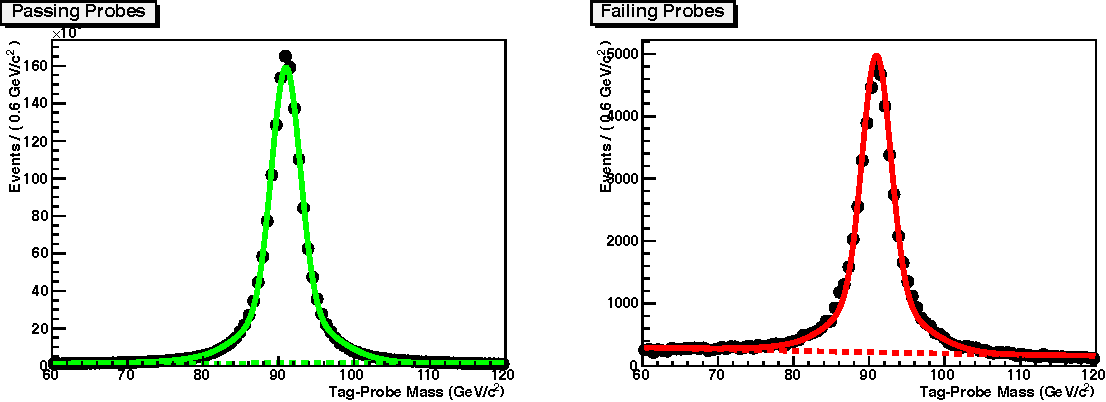
\includegraphics[width=\textwidth,clip=true]{matplotlib/efficiencies/fits-muonid-crop}
  \caption[Example fits to tag-probe muon pairs.]{Fits to the invariant mass spectrum of tag-probe pairs as defined for the muon identification efficiency measurement.  Pairs where the probe passes the identification criteria are shown on the left while pairs where the probe fails the identification criteria are shown on the right.  In each plot, the dashed line shows the linear fit to non-peaking background while the solid line shows the fit to genuine \ztomumu decays (Gaussian plus exponential).}
  \label{fig:muon-fits}
\end{figure*}

For muons, we consider the same efficiencies as above, but also \efftrk{} and \effsta{}, the efficiencies to reconstruct a track in the tracker given a stand-alone muon and to reconstruct a stand-alone muon given a track in the tracker, respectively.  The two measurements are assumed to be completely independent.  The total efficiency, then, is:
\begin{equation}
  \label{eq:factorized-eff-muon}
  \efftot = \efftrk \cdot \effsta \cdot \effid \cdot \effiso \cdot \effhlt.
\end{equation}
Results are given in Table~\ref{tab:muon-efficiencies}

We are also interested in understanding the frequency with which these electron and muon selection criteria incorrectly identify jets as leptons.  The misidentification rate is investigated in Sec.~\ref{sec:matrix-method} as part of a larger data-driven method to estimate the background contribution from \Zjets{} events.

